Early on, we considered car parking an amenity that had to be included on
Magpie's interface. Through our search of publicly available datasets, we were
unable to find any information on public, on the street or private parking
spaces in Ireland.

Thus, we settled on creating our own dataset of car parking spots in Dublin
using a novel machine learning approach.
This approach is divided into 3 main steps:
\begin{enumerate}
  \item Car detection on satellite images
  \item Parking detection using custom road mask
  \item Classification \& evaluation of the parking spots
\end{enumerate}
\subsubsection{YOLO model used for car detection}
YOLO (You Only Look Once) is an object detection and image segmentation model
launched in 2015 which quickly gained popularity for its high speed and
accuracy.

We were introduced to YOLO on Label Studio, an image labelling software used for
image recognition \& detection tasks. There is an extension called ML Backend on
the platform which can be used to automate the labelling process using an
integration of the YOLOv5 model. However, this extension was not working as
intended which caused us to pivot towards Ultralytics, the company behind the
YOLO models.

Several papers focusing on object detection cited YOLO over other popular models
such as (\cite{firedetectionYOLO}) and (\cite{polypdetectionYOLO}). A key
challenge that influences the choice of model for the object detection task is
effectively managing fluctuations in image resolutions and aspect ratios, as
well as the computational resources required to run image detection models.

There are two main types of models for object detection tasks: single stage and
two-stage. The figure below from \cite{singlevstwodetectorimg} illustrates the
process for both.

%single vs two stage model process
\begin{figure}[htbp]
  \centering
  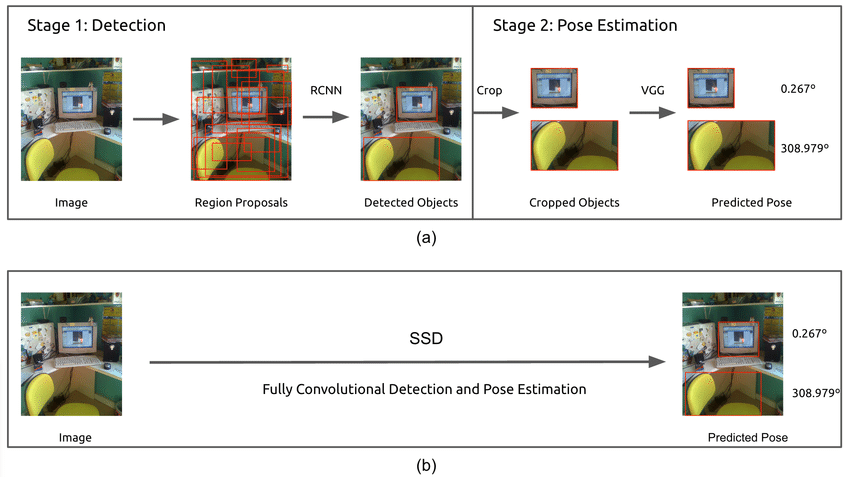
\includegraphics[width=0.7\textwidth]{images/single-vs-two-stage-obj-detector.png}
  \caption{Single vs Two-Stage Object Detection Process}
\end{figure}

\newpage{}
\textbf{Single stage} object detector models processes an image through a
feature extractor using a CNN (Convolutional Neural Network) and then directly
uses the extracted features for classification and regression of bounding boxes.
These models are very fast which is why they are popular for real-time object
detection tasks; however their accuracy performance can sometimes be poor.
Examples of single stage models are SSD, YOLO and RefineDet
(\cite{YOLOversionsliterature}.)

\textbf{Two stage} object detector models divides the process into two main
steps. First, it extracts features from the image using a CNN, then selects
regions of interests that will only be used for classification and regression of
bounding boxes. These models are much more accurate than one stage detectors and
are used for tasks where accuracy is prioritized over speed in the medical field
for example RCNN, Fast-RCNN and Faster-RCNN(\cite{singlevstwostagedetectors}).

For the scope of this project, we chose to continue with the YOLO models because
of their speed, their scalability and their lack of computational resources.

We experimented with different versions of the YOLOv5 model, then slowly
levelled up the versions up to version 8.  The YOLOv8 model has been pre-trained
on the COCO (Common Object in Context) dataset, a popular large scale dataset
with 200,000 images across 80 object categories commonly used for benchmarking
computer vision models (\cite{cocodataset}).

We monitored metrics such as mAP (mean Average Precision), F1-score and the
false positive rate. The figure below shows the metrics of the model as we
iteratively experimented up the version chain.

%model metrics graph
\begin{figure}[htbp]
  \centering
  \includegraphics[width=0.85\textwidth]{images/YOLO-results.png}
  \caption{YOLO Model training graph}
\end{figure}

We ended the object detection modelling training with the YOLOv8 - Oriented
Bounding Boxes (OBB).
Oriented bounding boxes are a newer type of bounding box where the bounding box
capture the orientation of the object providing a more accurate fit of the
object. They are defined by 5 parameters (center xy, width, height and rotation
angle) and capture the object's spatial orientation more precisely, reducing
overlap and improving the robustness of the object detection model
(\cite{obblit}).

\newpage{}
Below you can see the difference in bounding boxes between the labelled image
used for the non-OBB YOLOv5 \& YOLOv8 iterations versus the OBB YOLOv8.

%obb vs non obb bounding boxes
\begin{figure}[htbp]
  \centering
  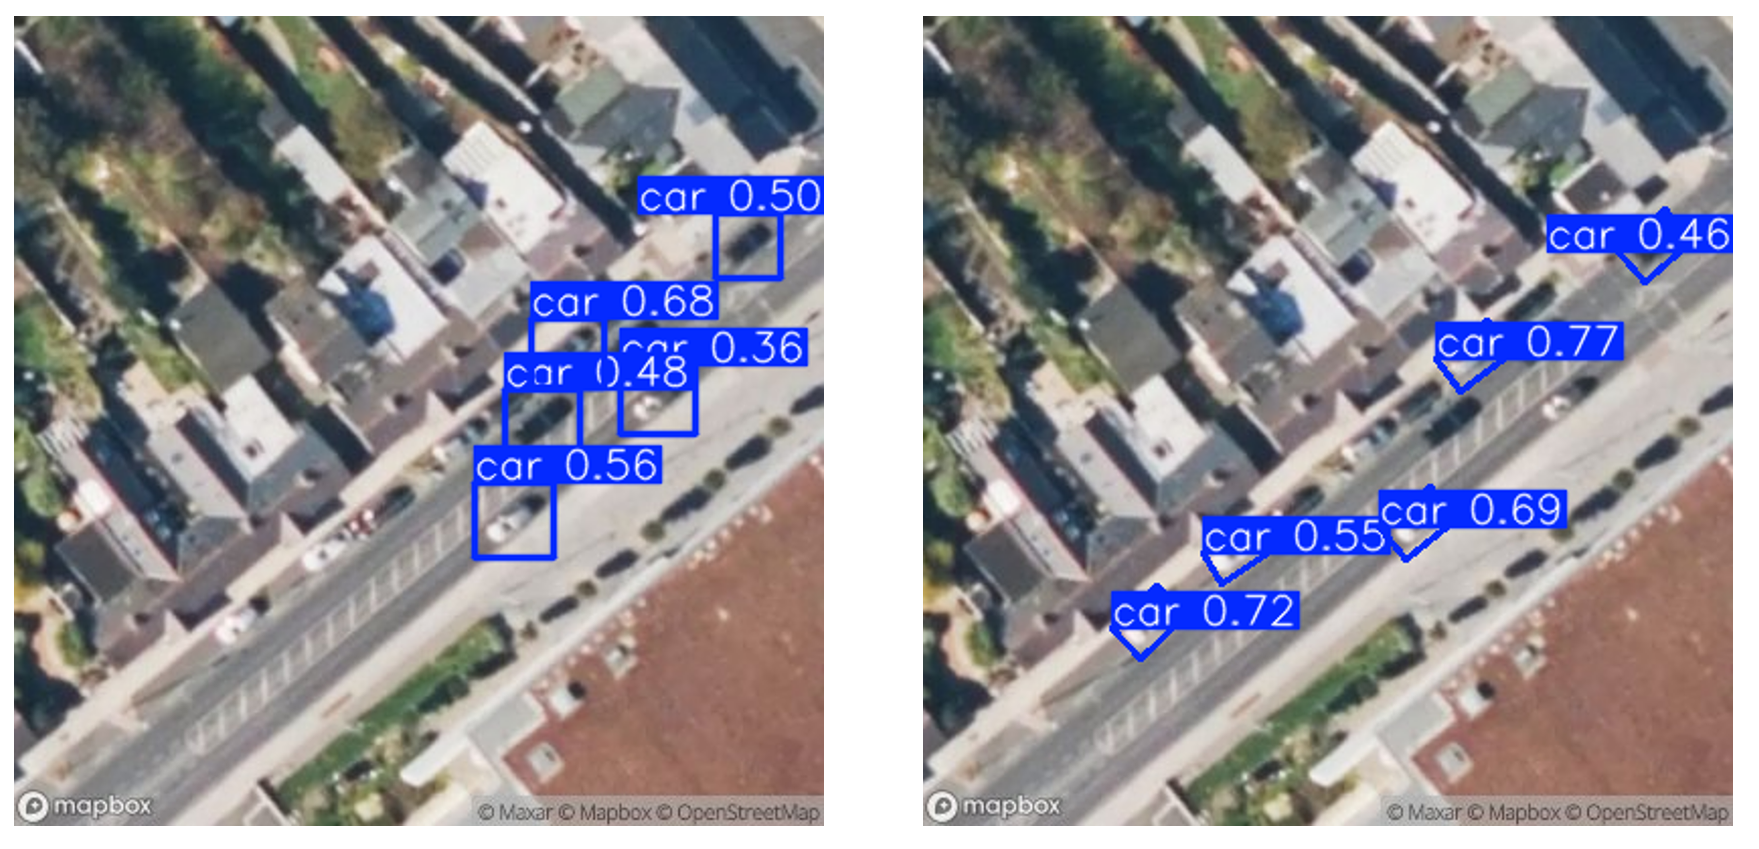
\includegraphics[width=0.85\textwidth]{images/obb-vs-nonobb-img.png}
  \caption{Non-OBB labels (left) versus OBB labels (right)}
\end{figure}

Lasly, the YOLOv8-OBB model was trained on the settings below:

\begin{listing}[htbp]
  \centering
  \begin{minted}{python3}
train_results_obb = YOLO8s_obb_model.train(data=data_config,
              epochs=35,
              patience=15,
              optimizer="AdamW",    # Adam + weight decay for less overfitting
              val=True, # validate during training
              seed=1,
              imgsz=416,
              batch=16,
              cache="disk",
              )
  \end{minted}
  \caption{YOLOv8-OBB model training settings}
\end{listing}

The weights of the YOLOv8-OBB model were then saved and used to identify parked
cars on over 18,000 satellite images spanning Dublin City. These images are then
used to identify parking spots.

\newpage{}
\subsubsection{Parking spot detection}
Subsequently, to identify the parking spots in each satellite image, the cars
detected by the YOLO model are classified into on the road or parked, based on a
road mask.

Many different iterations of the road mask were used, the main iterations and
their differences are explained and shown below in Figure 20.

\begin{figure}[htbp]
  \centering{}
  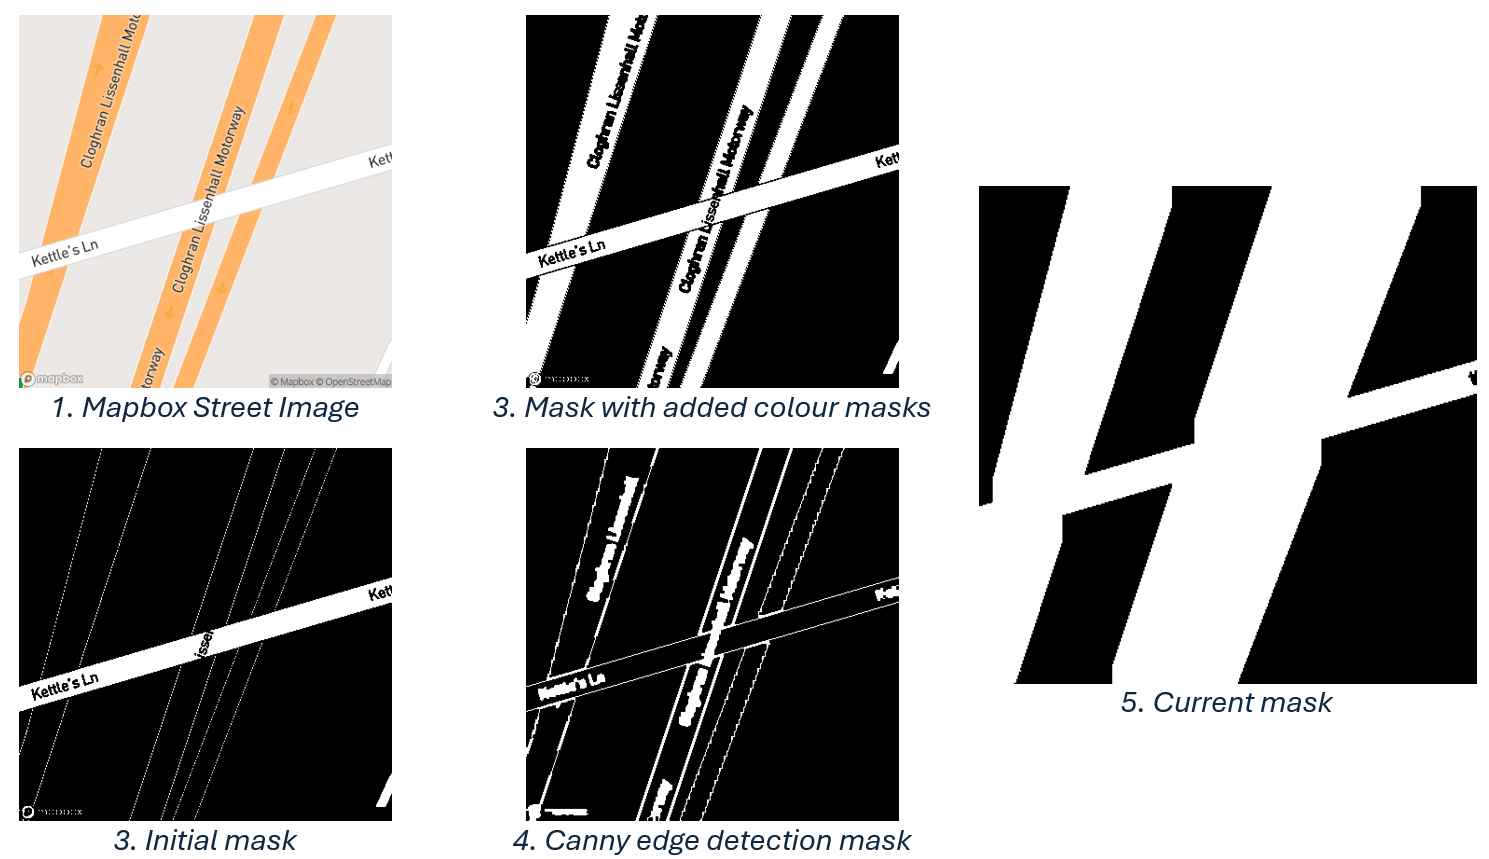
\includegraphics[width=0.7\textwidth]{images/road-mask-iteration.png}
  \caption{Different Iterations of the Road Mask}
  \label{fig:mask_iterations}
\end{figure}

The original mask was a very simple binary mask which identified the road pixels
by their color, as the majority of roads were depicted in white and darkened the
rest of the pixels in the image.

Through testing and thoroughly analysing the Mapbox Streets images, motorways
and national roads were discovered to be depicted in yellow or orange.
Therefore, two additional color masks (for orange and yellow) were concatenated
to the original binary mask through bitwise operations.

To refine the mask, and reduce misclassification errors, additional annotations
contained on the Mapbox Streets images such as street names and white dotted
lines which denote a multitude of things (foot paths, planter boxes, pedestrian
crosswalks, football fields delimitations, etc. ) were removed through
morphological operations, leaving only a plain white line for each road. A
number of different kernel sizes, different contour thresholds and other
parameters were tested to achieve the optimal removal of the street names and
additional annotations.

A different approach using Canny Edge Detection was tested, however due to the
nature of the Mapbox Streets images, the edges picked up were not significant
and the overall performances was much worse than the current mask at the time.

A final improvement to the mask was made to avoid certain misclassification due
to the Mapbox Streets road width not correctly reflecting all the lanes of the
road and therefore classifying on the road cars as parked. This issue was most
prominent for motorways and national roads and was resolved by enlarging those
roads using a dilation technique. Multiple different kernel sizes, different
number of iterations and kernels of different sizes applied consecutively were
tested to find the optimal solution.

\newpage{}

\subsubsection{Parking spot classification}
The process of classifying the parking spots has been split into 3 steps:
\begin{enumerate}
  \item Classify initial spots as \emph{on the road} or {parked}
  \item Identify additional \emph{empty} parking spots
  \item Classify all identified spots in \emph{3 classes}
\end{enumerate}

\textbf{Step 1 - Classifying into on the road or parked}

The cars detected by the YOLO model are then sorted into on the road or parked
based on the road mask previously generated, which is explained in more detail
below.

The model's predictions which are lower than the confidence threshold of 0.4 are
discarded as they are more likely to be misclassifications, such as chimneys or
roof pieces which were often misclassified as cars, which can be seen below on
the second image of Figure 21.

\begin{figure}[htbp]
  \centering
  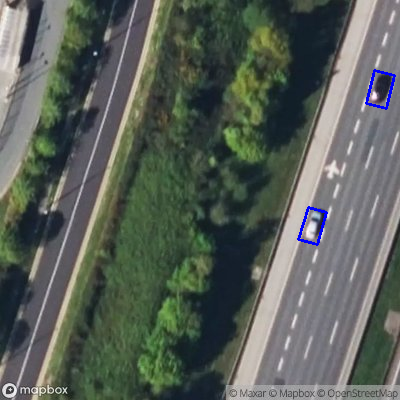
\includegraphics[width=0.30\textwidth]{images/road_mask_classification1.png}
  \hfill
  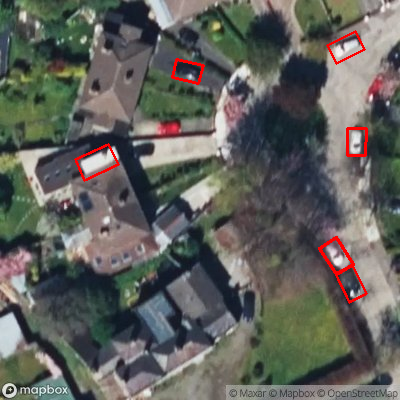
\includegraphics[width=0.30\textwidth]{images/road_mask_classification2.png}
  \hfill
  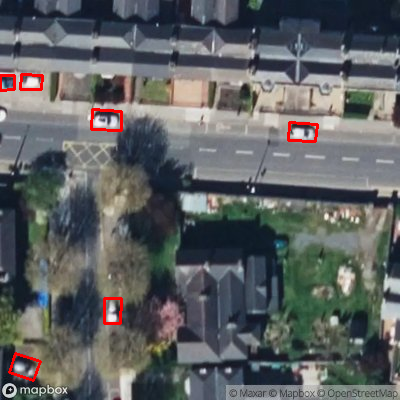
\includegraphics[width=0.30\textwidth]{images/road_mask_classification3.png}
  \caption{Classification of cars as on the road or parked: (left) Initial Classification, (center) Intermediate Stage, (right) Final Classification.}
  \label{fig:road_mask_classification}
\end{figure}

A bounding box for each of the model's predictions is computed from the center
pixel coordinates, the width and the height returned from the model. The overlap
between the bounding box and the road pixels is calculated, and if the overlap
is higher than the threshold of 0.5, the prediction is discarded, keeping only
the parked cars. Different thresholds were tested as well, however overall a
harsher threshold works better given that these detections are used later on for
the empty parking detection.

For each of the model's predictions for parked cars, the center pixels
coordinates are mapped to geographic coordinates (longitude and latitude), and
the width, height, rotation and orientation based on the angle are saved. The
horizontal orientation is assigned for spots that have a rotational angle in
degrees ranging between -45 and 45 or between 135 and 225, while the vertical
orientation is assigned to the remaining spots that do not fit the criteria.

For testing and debugging purposes, all the bounding boxes of the cars found by
the model are drawn onto the satellite image, on the road cars are drawn in blue
while parked cars are drawn in \textbf{red} as seen above in
Figure 21.

\newpage{}

\textbf{Step 2: Detecting unoccupied parking spots}

We have managed to identify occupied parking spots, therefore it is necessary to
identify unoccupied ones to offer a more comprehensive view of car parking in
Dublin city.

Unoccupied parking spots are detected between parked cars in each image, based on the
parked cars detected by the YOLO model and classified using the road mask.

A number of different variations and calculation techniques were tested out,
however only the final version will be explained below.

Average parking spot width and length in pixels are calculated for each image,
to draw the empty spots more uniformly. Average parking spot width and length in
meters are set to 3.05 as found to be the optimal value through testing
accounting for the variations in size.

Setting this value avoids misclassifications, as previously the average width and
length in meters were calculated dynamically, however in cases where the
averages were lesser than 3, spots tended to overlap.

The parked cars detected are then sorted by latitude for horizontally aligned
cars and by longitude for vertically aligned cars, to identify gaps between
consecutive cars. For each pair of consecutive spots, the distance in meters in
between them is calculated. The gap is adjusted to account for the half cars on
both sides, as the coordinates of the parked car represent the center of the
car. For the gaps smaller than the maximum gap threshold of 12 meters and larger
than the average size of a car, where there is enough space to fit 1 or more
car, and where the angle deviation is smaller than a threshold of 35 degrees, to
ensure the spots are sufficiently aligned, the number of cars that fit into the
gap is calculated.

Based on the number of unoccupied spots found, the coordinates for those empty spots
are calculated to be aligned with the 2 consecutive cars and then added to a
list of empty spots detected.

Afterwards, spots where the distance between them is smaller than a threshold of
1 meter are removed.

Additionally, spots coinciding with cars identified by the YOLO model, where the
distance between them is smaller than 1.25 meters are removed from the unoccupied
spots found. Spots that overlap with the road are filtered out in a similar
manner to the classification done by the road mask.

Following the detection of all the unoccupied spots, the bounding boxes
corresponding to each spot are drawn onto the satellite image in \textbf{green} as shown
in Figure 22.

\begin{figure}[htbp]
  \centering
  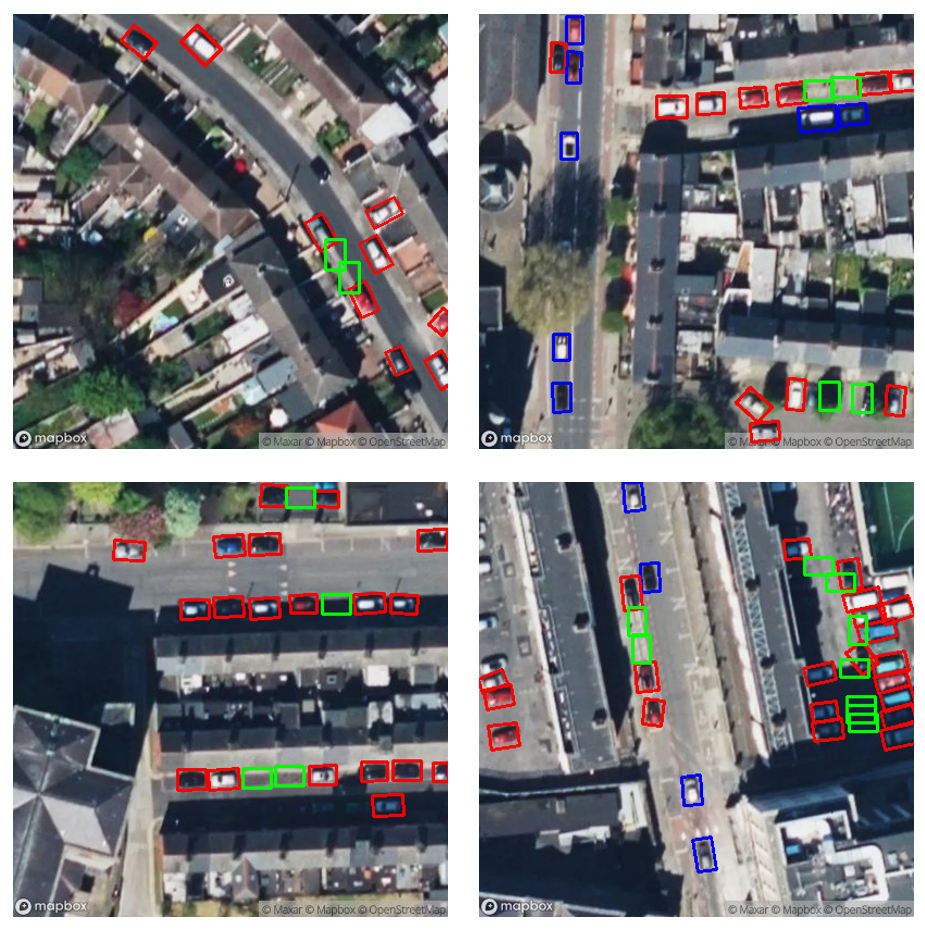
\includegraphics[width=0.9\textwidth]{images/empty-parking-detection.png}
  \caption{Empty Parking Spot Detection}
  \label{fig:Empty_parking_detection}
\end{figure}

\newpage{}

\textbf{Step 3: Classification of all spots detected}
Both the parked cars identified by the model and the unoccupied parking spots are
then classified into 3 different classes: \emph{public} (on the street parking),
private (residential parking) and parking lot, based on their proximity to the
nearest road.

\hspace{2em}\textbf{Public \& private parking spots}

Parking spots are classified as \emph{public} if the proximity to the nearest
road is less than a pixel threshold of 30, otherwise the parking spots are
considered \emph{private}.

This optimal threshold was found through extensive testing on a test
set containing various edge cases.

\hspace{2em}\textbf{Parking lot spots}

Parking spots are classified as parking lots, when clusters of 18 or more spots
are identified in an image. Larger clusters are prioritized as parking lots to
minimize the risk of misclassifying residential areas as parking lots.

Multiple different clustering approaches were tested out to cluster spots
together, such as DBSCAN, HDBSCAN and OPTICS.

Overall DBSCAN performed the best and the quickest out of all the clustering
algorithms, given that some images contained very few parking spots, meaning
clustering was only significant in cases with a minimum number of parking spots.

Through testing, the optimal hyperparmeters found for DBSCAN are \texttt{eps} :
55 and \texttt{min\_samples} : 5, which allow the correct identification of the
clusters, avoiding misclassifications of residential areas with many cars as
parking lots, which was a common misclassification initially, when the
hyperparameters and thresholds were not set correctly.

\texttt{eps} refers to the maximum distance between two points for them to be
considered as neighbors and \texttt{min\_samples} refers to the minimum number
of points required to form a cluster.

Using HDBSCAN and OPTICS required a minimum number of samples larger or equal to
2. However, not all images contained at least 2 parked cars therefore clustering using
those algorithms was not possible in all cases. A value of -1 was assigned to the
spots belonging to no clusters similarly to the default behaviour of DBSCAN.

Clustering using HDBSCAN gave slightly lower results to DBSCAN, while OPTICS
only found smaller clusters which were not as significant and not particularly
helpful to classify the spots into the parking lot category.

Afterwards, clusters and classification labels are drawn onto the satellite
image. The clusters are color coded and denoted as a circle at the center of the
bounding box, while the classification label is written to the right of the
bounding box. The private class in written in red, public in green and parking
lot in white as seen below in Figure 23.

\begin{figure}[htbp]
  \centering
  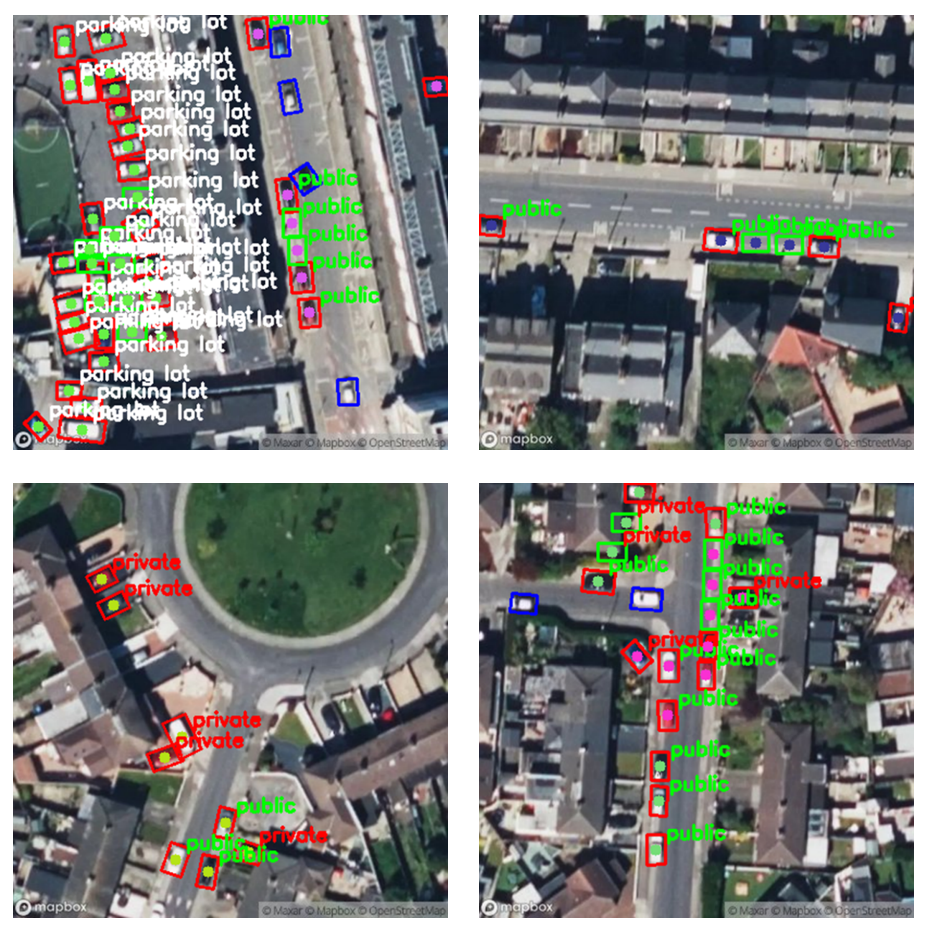
\includegraphics[width=0.9\textwidth]{images/classification-cars.png}
  \caption{Classification of all spots into private, public and parking lot}
  \label{fig:classification_all_spots}
\end{figure}

\newpage{}

\subsubsection{Evaluation of each submodule of the parking detection model}
Each major section of the parking detection model was evaluated individually in
order to assess the overall performance. The results will be presented for each
section below.

\textbf{Evaluation of the YOLOv8-OBB model}\\
The YOLOv8-OBB model was evaluated on a validation set of 51 images, where
precision, recall, accuracy, mean average precision (mAP@50) and F1-score were
computed. These were the scores below:
%YOLOv8 obb results
\begin{table}[htbp]
  \centering
  \begin{tabular}{|p{0.18\textwidth}|p{0.1\textwidth}|p{0.1\textwidth}|p{0.1\textwidth}|p{0.1\textwidth}|p{0.1\textwidth}|p{0.12\textwidth}|}
    \hline
    \textbf{Model} & \textbf{Accuracy} & \textbf{Precision} & \textbf{Recall} & \textbf{F1-score} & \textbf{mAP@50} & \textbf{Conf threshold} \\
    \hline
    YOLOv8-OBB     & 94\%              & 100\%              & 99\%            & 91\%              & 94\%            & 35\%                    \\
    \hline
  \end{tabular}
  \caption{YOLOv8-OBB model results}
\end{table}

The model obtains near perfect precision and recall on the validation data set
meaning it is very good at correctly identifying the majority of true positives
and preventing false positives. However, the lower f1 score of 91\% highlights
the slight imbalance between precision and recall. Additionally, the confidence
threshold is based on the F1-score, suggesting that the model performs at a
level where precision and recall are balanced best closer to 30\%. This
indicates that our model is not strict.

Although the overall metrics obtained are quite high, it is important to
consider that, the validation and training data are not very large, therefore
impacting overall model performance to identify cars in a larger detection set.

\textbf{Evaluation of the classification of cars into on the road or parked}

The classification of cars into on the road or parked by the road mask is
evaluated in the \texttt{evaluate\_road\_mask.py} Python script. The
classification is evaluated on the following metrics commonly used for object
detection tasks: Average Intersection over Union (IoU), Balanced Accuracy and
Precision, Recall, F1 Score, Accuracy, Specificity per class.

These metrics are defined in detail as follows.

The IoU is calculated as the overlap between the predicted bounding box \( B_p
\) and the ground truth bounding box \( B_g \), divided by their union:

\[
  \text{IoU} = \frac{|B_p \cap B_g|}{|B_p \cup B_g|}
\]

The Average IoU is defined as the mean IoU across all detections:

\[
  \text{Average IoU} = \frac{1}{N} \sum_{i=1}^{N} \text{IoU}_i
\]

where \( N \) is the total number of detections.

\newpage{}

Precision is defined as the ratio of true positives (TP) and the sum of true
positives and false positives (FP):

\[
  \text{Precision} = \frac{\text{TP}}{\text{TP} + \text{FP}}
\]

Recall is defined as the ratio of true positives (TP) and the sum of true
positives and false negatives (FN):

\[
  \text{Recall} = \frac{\text{TP}}{\text{TP} + \text{FN}}
\]

The F1 Score is defined as the harmonic mean of precision and recall:

\[
  \text{F1 Score} = 2 \cdot \frac{\text{Precision} \cdot \text{Recall}}{\text{Precision} + \text{Recall}}
\]

Accuracy is defined as the proportion of correct predictions (TP and TN) out of
all the predictions:

\[
  \text{Accuracy} = \frac{\text{TP} + \text{TN}}{\text{TP} + \text{TN} + \text{FP} + \text{FN}}
\]

Balanced Accuracy is defined as the average of Sensitivity (or Recall) and
Specificity:

\[
  \text{Balanced Accuracy} = \frac{\text{Sensitivity} + \text{Specificity}}{2}
\]

where:
\[
  \text{Sensitivity/Recall} = \frac{\text{TP}}{\text{TP} + \text{FN}}, \quad
  \text{Specificity} = \frac{\text{TN}}{\text{TN} + \text{FP}}
\]

These metrics are then saved in a csv file for each test image as well as the
overall average metrics on the entire test set.

A test set of 50 images was carefully selected to include edge cases and
difficult cases and then consistently labelled in Label Studio as seen in
Figure~\ref{fig:LabelStudio_test_set}. The labels are drawn without rotation to
ensure the maximum overlap, as the labels are exported to \texttt{txt} format
and include only the pixel coordinates, width and  height of the bounding boxes
annotated.

\begin{figure}[htbp]
  \centering
  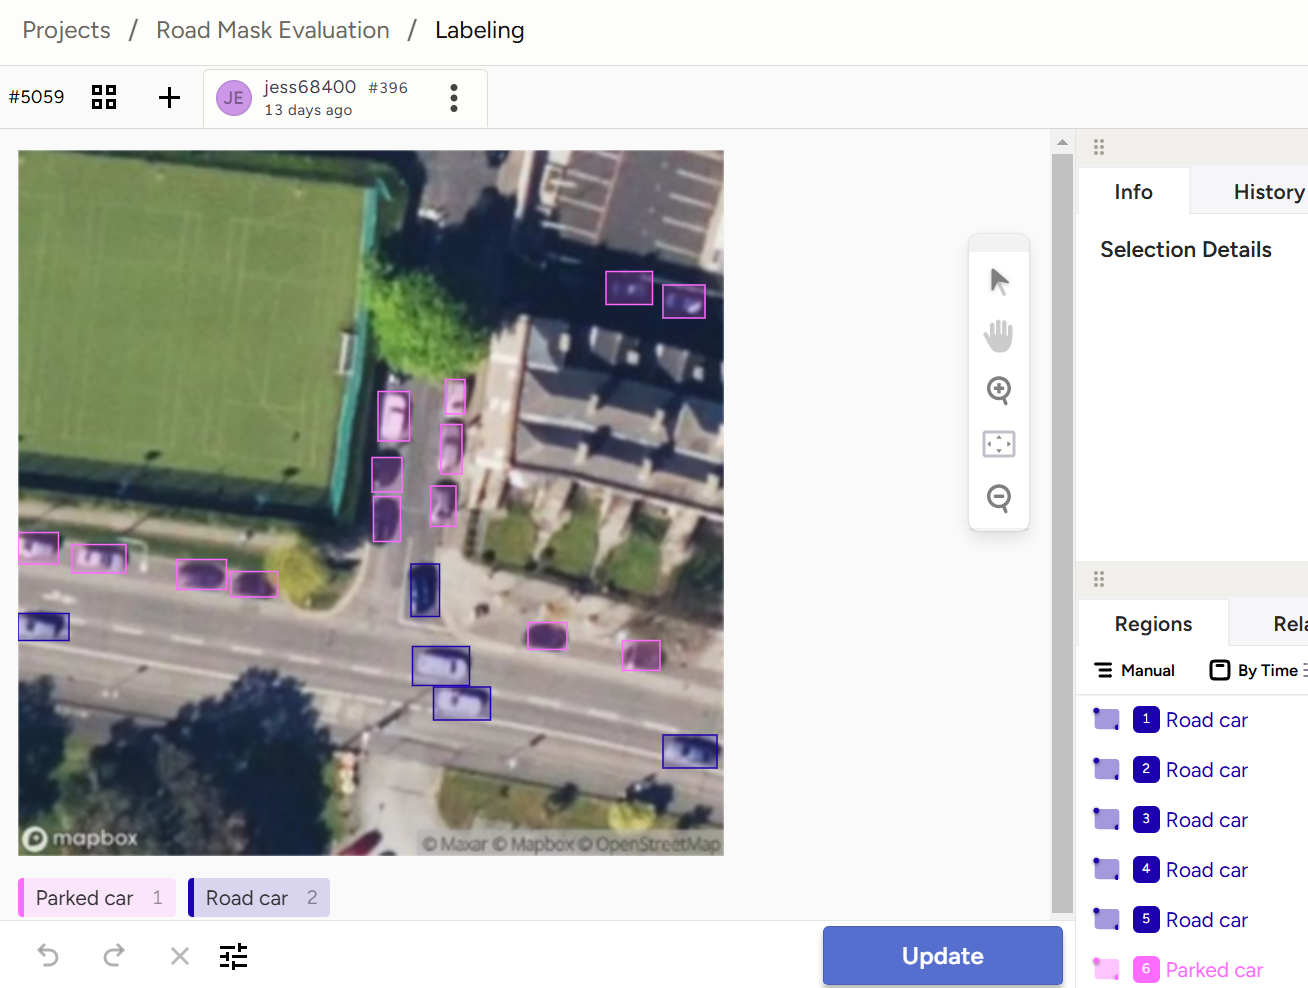
\includegraphics[width=0.9\textwidth]{images/label_studio4.png}
  \caption{Road mask classification test set images being annotated in Label Studio}
  \label{fig:LabelStudio_test_set}
\end{figure}

\newpage{}


The overall results on test set are presented below in Table 2.

\begin{table}[htbp]
  \centering
  \begin{tabular}{|l|c|c|}
    \hline
    \textbf{Metric}           & \textbf{Parked} & \textbf{Road} \\ \hline
    Average IoU               & 0.66            & 0.66          \\ \hline
    Average Balanced Accuracy & 0.58            & 0.58          \\ \hline
    Average Precision         & 0.70            & 0.90          \\ \hline
    Average Recall            & 0.75            & 0.67          \\ \hline
    Average F1 Score          & 0.59            & 0.54          \\ \hline
    Average Accuracy          & 0.69            & 0.64          \\ \hline
    Average Specificity       & 0.74            & 0.79          \\ \hline
  \end{tabular}
  \caption{Performance Metrics for Road Mask Classification}
  \label{tab:metrics1}
\end{table}

Precision and Recall are relatively high for both classes. Precision for the on
the road cars class is extremely high as the majority of the cars in the test
set were perfectly horizontally or vertically aligned, and given that the
rotation cannot be exported in label studio, the bounding box is drawn less
accurately unless if it is perfectly horizontally or vertically aligned.

\newpage{}

Similar papers that explore object detection for cars on satellite images
evaluate their experiment on more general metrics such as \emph{Average
  Precision (AP)} and \emph{Mean Average Precision (mAP)}.

AP represents the area under the precision-recall curve and mAP represents the
mean of the APs across all the different classes. These metrics provide a
broader overview of the model's performance as it is measured across varying
thresholds.

The results obtained on our model are not directly comparable, given that
precision, recall and f1 score are calculated for a fixed IoU threshold in our
evaluation.

Nevertheless, they are in line with \cite{similarresults}, who achieve a
\underline{precision of 0.75}, a \underline{recall of 0.66} and an \underline{f1
  score of 0.70} at the \underline{IoU threshold of 0.30}, for detecting parked
car on stereo satellite images.

The current road mask has a few outstanding problems, that are discussed further
below.

Firstly, not all street names are completely removed due certain factors such as
the Mapbox watermark and the length of the street name, the latter causing
identified cars on the road to be misclassified as parked.

Secondly, the Mapbox Streets images used to create the road mask do not
correctly reflect the width of the road for roads with multiple lanes, which
leads to certain cars on the road being misclassified as parked. This issue was
resolved for motorways as they are depicted in orange or yellow, making
it possible to distort the mask to cover more surface.

Another problem inherent to Mapbox Streets images is the Dublin Tunnel being
marked as above ground even though it is underground, leading to certain
misclassiifcations in that specific area.

Some images from the test set can be seen below in
Figure . The predicted parked cars are drawn in red while
the true labels are drawn in light pink. The predicted on the road cars are
drawn in blue while the true labels are drawn in cyan.

\begin{figure}[htbp]
  \centering
  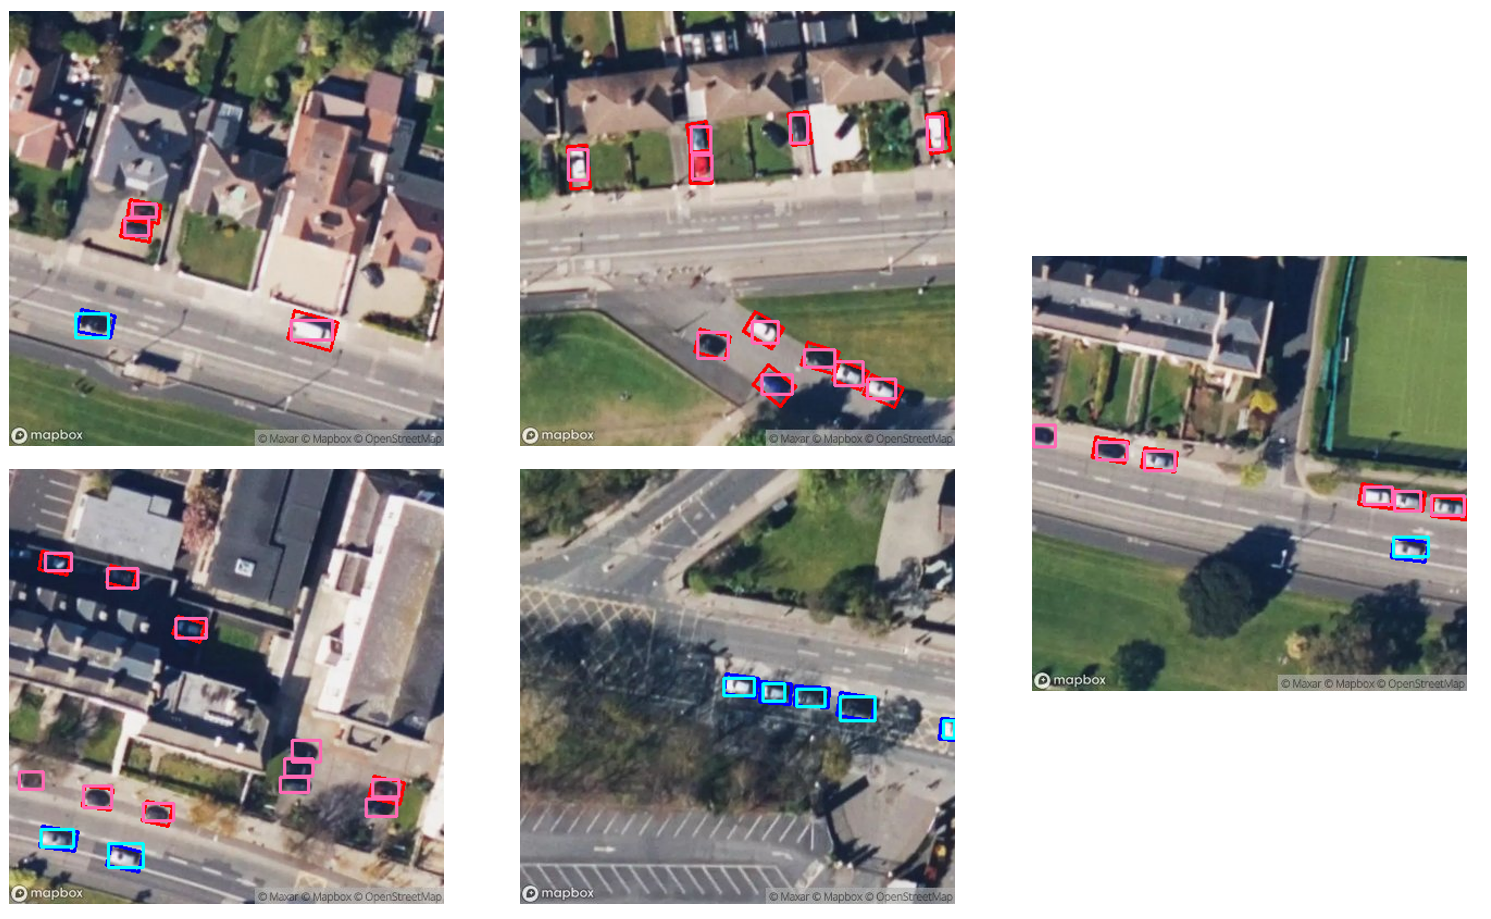
\includegraphics[width=0.8\textwidth]{images/road-mask-classification-test.png}
  \caption{Images from the Road Mask Classification Test Set}
  \label{tab:test_images1}
\end{figure}

\newpage{}

\textbf{Evaluation of the empty parking detection}

The empty parking detection logic is evaluated in the
\texttt{evaluate\_empty\_parking\_detection.py} Python script. The
classification is evaluated on the following metrics: Average IoU, Average
Precision, Average Recall, Average F1 Score, Average Orientation Accuracy,
Average Spot Detection Ratio (SDR), Average Spot Detection Error (SDE), Average
False Positive Rate (FPR), and Average False Negative Rate (FNR).

The additional metrics are defined as follows.

The Average Orientation Accuracy is defined as the ratio of the number of
predictions that correctly identify the orientation (either horizontal or
vertical) of the spots on the total number of true spots:

\[
  \text{Average Orientation Accuracy} = \frac{\text{Correct Orientation Predictions}}{\text{Total True Labels}}
  = \frac{N_{\text{correct\_orientation}}}{N_{\text{true\_labels}}}
\]

where \( N_{\text{correct\_orientation}} \) represents the number of predictions
with correct orientation, and \( N_{\text{true\_labels}} \) represents the total
number of true labels.

The Spot Detection Ratio is defined as the ratio of the number of predictions
and the total number of true labels:

\[
  \text{SDR} = \frac{N_{\text{predictions}}}{N_{\text{total\_true\_labels}}}
\]

where \( N_{\text{predictions}} \) is the total number of detected spots, and \(
N_{\text{total\_true\_labels}} \) is the total number of true labels.

The Spot Detection Error is defined as the absolute difference between the
number of predictions and the total number of true labels:

\[
  \text{SDE} = |N_{\text{predictions}} - N_{\text{total\_true\_labels}}|
\]

The False Positive Rate is defined as the proportion of incorrectly predicted
positives (FP) out of all the actual negatives:

\[
  \text{Average FPR} = \frac{\text{FP}}{\text{FP} + \text{TN}}
\]

The False Negative Rate is defined as the proportion of incorrectly predicted
negatives (FN) out of all the actual positives:

\[
  \text{Average FNR} = \frac{\text{FN}}{\text{TP} + \text{FN}}
\]

These metrics are then saved in a csv file for each test image as well as the
overall average metrics on the entire test set.

\newpage{}

Likewise a test set of 50 images was carefully selected and consistently
labelled in Label Studio, without rotation to ensure the maximum overlap. The
pixel coordinates, width and height of the annotated bounding boxes are
exported. The orientation of each bounding box, is calculated automatically in
the evaluation script when loading in the true labels.

Achieving a high IoU was a significant challenge, specifically in this section
of the model, as the positioning of the spots can be difficult to label
accurately. Indeed, it was difficult to identify if there was sufficient space
available to fit a car. To remedy this issue, the IoU threshold was lowered to
0.35, as there was still significant overlap visible when analysing the test
images.

The problems linked to the overlap, is equally due to the differences in
orientation as the true labels and the predictions are calculated differently.
For the true labels, the orientation is based on whether the width or length of
the spot is larger (the spots with larger width are labelled as horizontal and
the spots with larger length are labelled as vertical), while for the model's
predictions the orientation is based on the angle measurement.

The overall results on test set are presented below in Table 3.

\begin{table}[htbp]
  \centering
  \begin{tabular}{|l|c|}
    \hline
    \textbf{Metric}                    & \textbf{Value} \\ \hline
    Average IoU                        & 0.59           \\ \hline
    Average Precision                  & 0.77           \\ \hline
    Average Recall                     & 0.70           \\ \hline
    Average F1 Score                   & 0.69           \\ \hline
    Average Orientation Accuracy       & 0.64           \\ \hline
    Average Spot Detection Ratio (SDR) & 1.05           \\ \hline
    Average Spot Detection Error (SDE) & 1.44           \\ \hline
    Average False Positive Rate (FPR)  & 0.23           \\ \hline
    Average False Negative Rate (FNR)  & 0.22           \\ \hline
  \end{tabular}
  \caption{Performance Metrics for Empty Parking Detection}
  \label{tab:metrics2}
\end{table}

The Average Orientation Accuracy being somewhat low of only 0.64 is expected
because the orientation labels for the test set are calculated automatically
based on the width and length of the bounding box. On the other hand, the
orientation associated with the model’s prediction is based on the rotation.
This is illustrated below, the orientated label in \textbf{pink} and the
non-oriented one in \textbf{green}.

\begin{figure}[htbp]
  \centering
  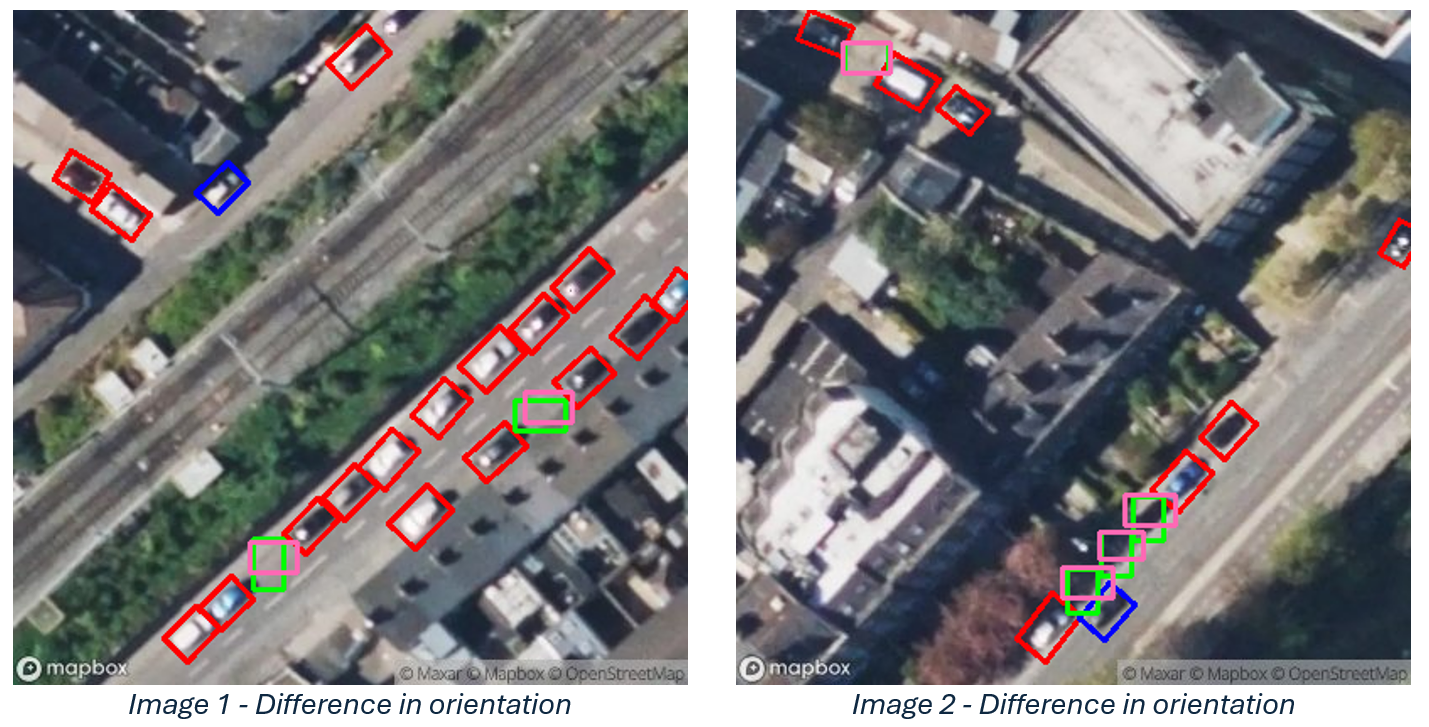
\includegraphics[width=0.6\textwidth]{images/empty-detection-orientation.png}
  \caption{Empty detection test set - True label vs Predicted label}
\end{figure}

\newpage{}

The results achieved are similar to other articles performing car detection on
satellite imagery such as \cite{similarresults}.

The main reason unoccupied parking spots are not detected is because cars are
classified as on the road by the road mask and the empty parking detection logic
only applies to parked cars. This is illustrated in the figure below.
\begin{figure}[htbp]
  \centering
  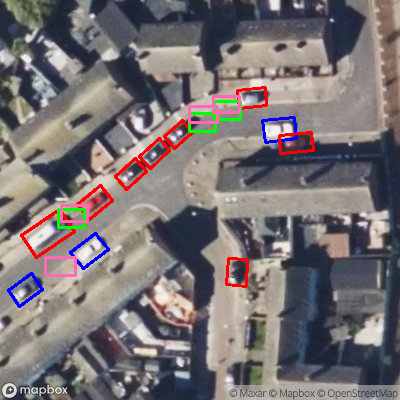
\includegraphics[width=0.5\textwidth]{images/empty-detection-orientation2.png}
  \caption{Empty detection test set - True label vs Predicted label}
\end{figure}

\textbf{Evaluation of classification of spots into private, public \& parking lot}
The classification of the spots detected into private, public and parking lot is
evaluated in the \texttt{evaluate\_classification\_of\_spots.py} Python script.
The classification is evaluated on the following metrics as defined previously:
Average IoU, Balanced Accuracy and Precision, Recall, F1 Score, Accuracy,
Specificity per class. These metrics are saved in a csv file for each test image
as well as the overall average metrics on the entire test set.

Similarly, a test set of 50 images was carefully selected and consistently
labelled in Label Studio, without rotation to ensure the maximum overlap.

The overall results on the test set are presented below in Table 4.

\begin{table}[htbp]
  \centering
  \begin{tabular}{|l|c|c|c|}
    \hline
    \textbf{Metric}           & \textbf{Public} & \textbf{Private} & \textbf{Parking Lot} \\ \hline
    Average IoU               & 0.60            & 0.60             & 0.60                 \\ \hline
    Average Balanced Accuracy & 0.57            & 0.57             & 0.57                 \\ \hline
    Average Precision         & 0.73            & 0.65             & 0.59                 \\ \hline
    Average Recall            & 0.72            & 0.75             & 0.74                 \\ \hline
    Average F1 Score          & 0.68            & 0.62             & 0.61                 \\ \hline
    Average Accuracy          & 0.67            & 0.54             & 0.63                 \\ \hline
    Average Specificity       & 0.59            & 0.54             & 0.41                 \\ \hline
  \end{tabular}
  \caption{Performance Metrics for Parking Spot Classification}
  \label{tab:metrics3}
\end{table}

\newpage{}

The performance is similar for all 3 classes, however for the parking lot class
more false positives are present, given that having many bounding boxes
clustered together creates more unpredictability adding more additional spots.

The results presented above are in line with other articles performing car
detection on satellite imagery such as \cite{similarresults}.

The main outstanding problem for this section is residential areas which are
very rarely misclassified as parking lots. Additionally, in cases where public
spots are quite far from the nearest road, the spots are misclassified as
private, which is not a major issue.

Another point worth noting is that smaller parking lots with less than 18 spots
are not detected though that is intentional and by design in order to focus on
larger parking lots and avoid misclassifications.

A few images from the test set are shown below in Figure 28.
The predicted public spots are drawn in green while the true labels are in dark
green. The predicted private spots are highlighted in red while the true labels
are in light pink. The predicted parking lot spots are shown in blue while the
true labels are in cyan.

\begin{figure}[htbp]
  \centering
  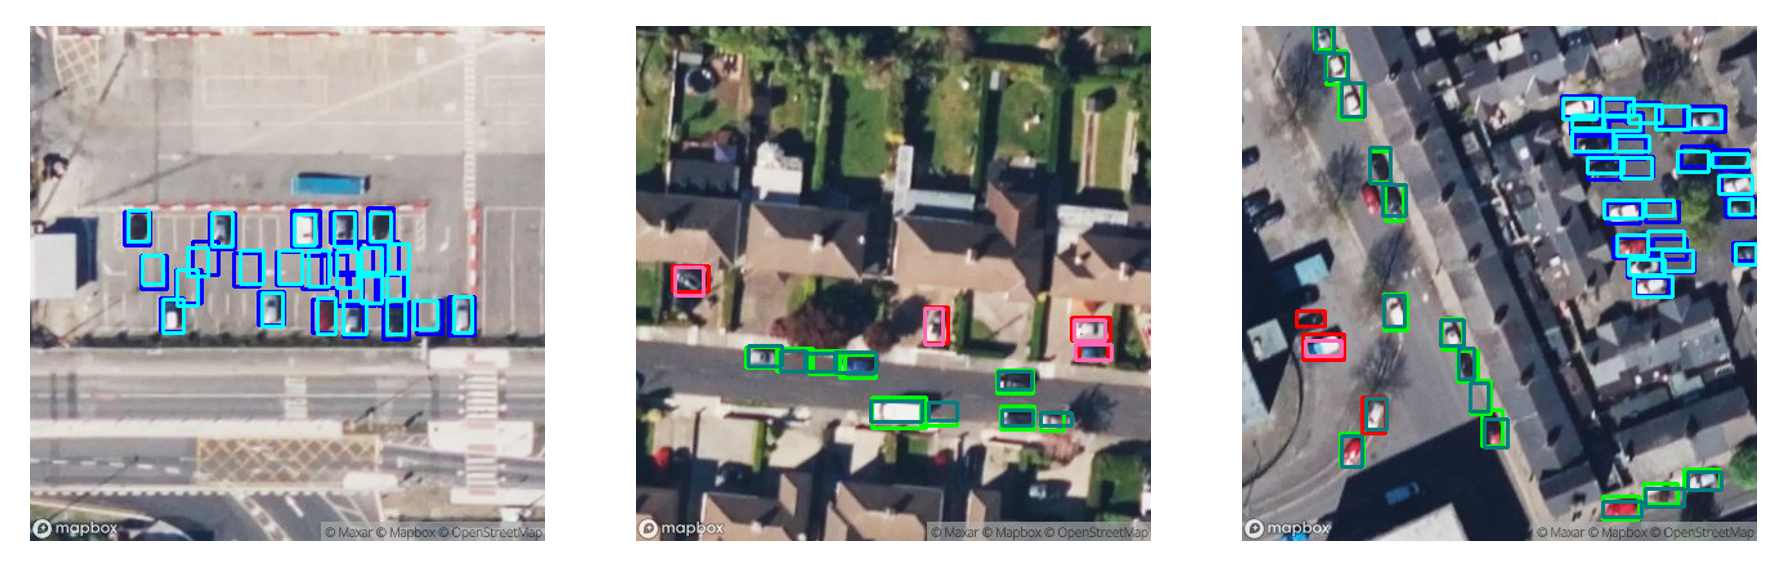
\includegraphics[width=0.9\textwidth]{images/classification-spots-test.png}
  \caption{Classification of spots test set - True label vs Predicted label}
\end{figure}

\newpage{}

\subsubsection{Integration with Magpie system}
Once all the parking spots have been identified, their longitude, latitude and
class are saved to a csv file. Potential spot duplicates are dropped, and
parking zones and associated tariffs are added.

Parking zone and tariff were obtained by manipulating the map shown in the
figure below in QGIS, a geographic information system used for working with
spatial data. Polygons were drawn on a raster layer, and associated id, zone
name and tariff were defined before being exported as a geojson.

Dublin City Council defines different parking zones by color, based on their
high to moderate demand which changes the price per zone as seen below in Figure
24.

\begin{figure}[htbp]
  \centering
  \begin{minipage}{0.45\textwidth}
    \centering
    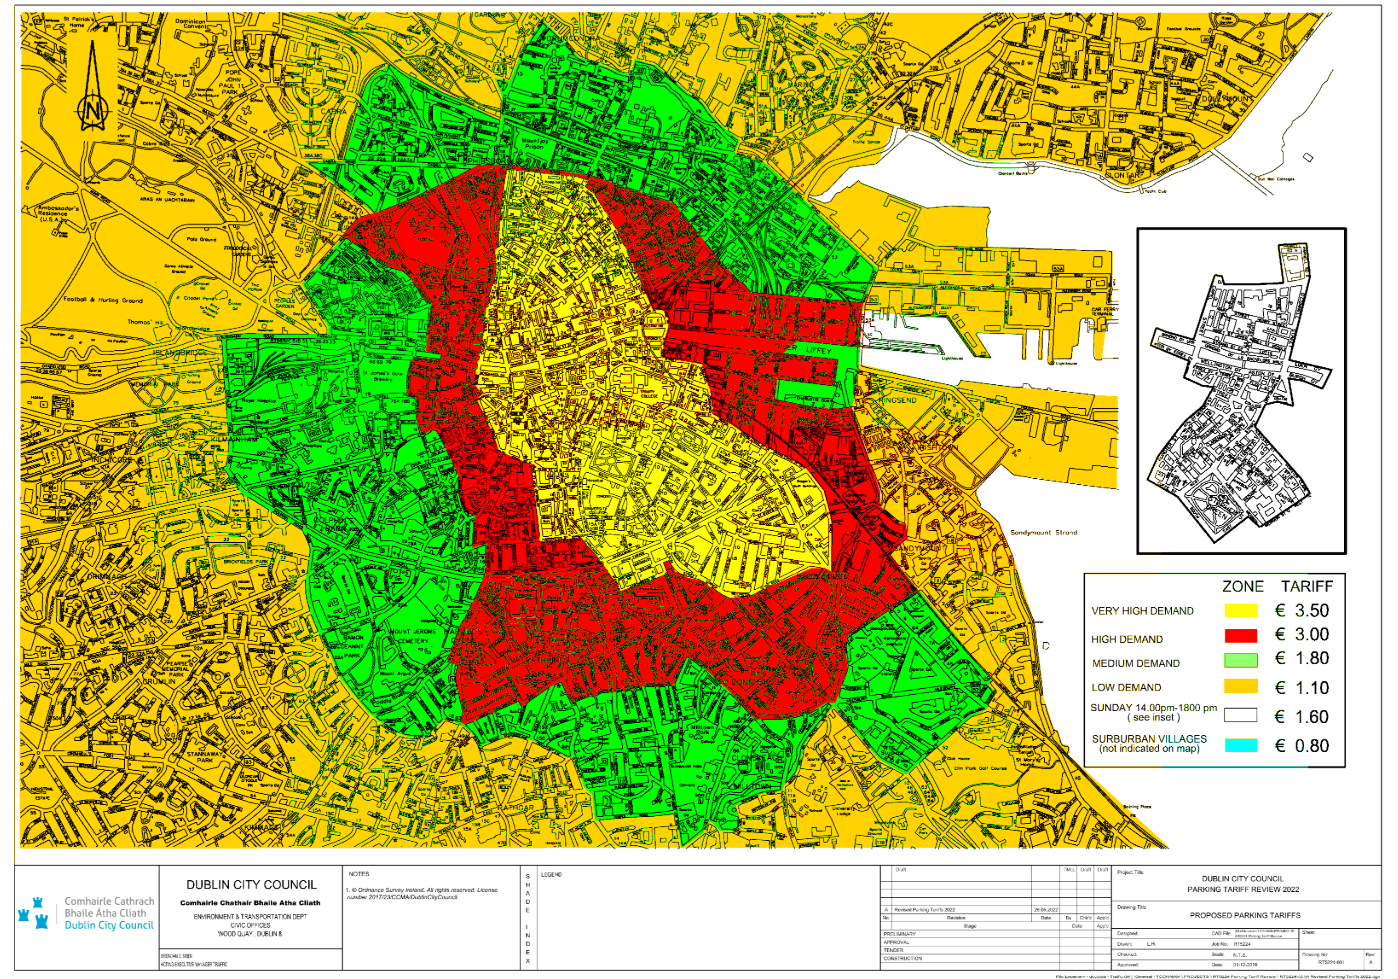
\includegraphics[width=\textwidth]{images/Parking_zones_map.png}
  \end{minipage}
  \hfill
  \begin{minipage}{0.45\textwidth}
    \centering
    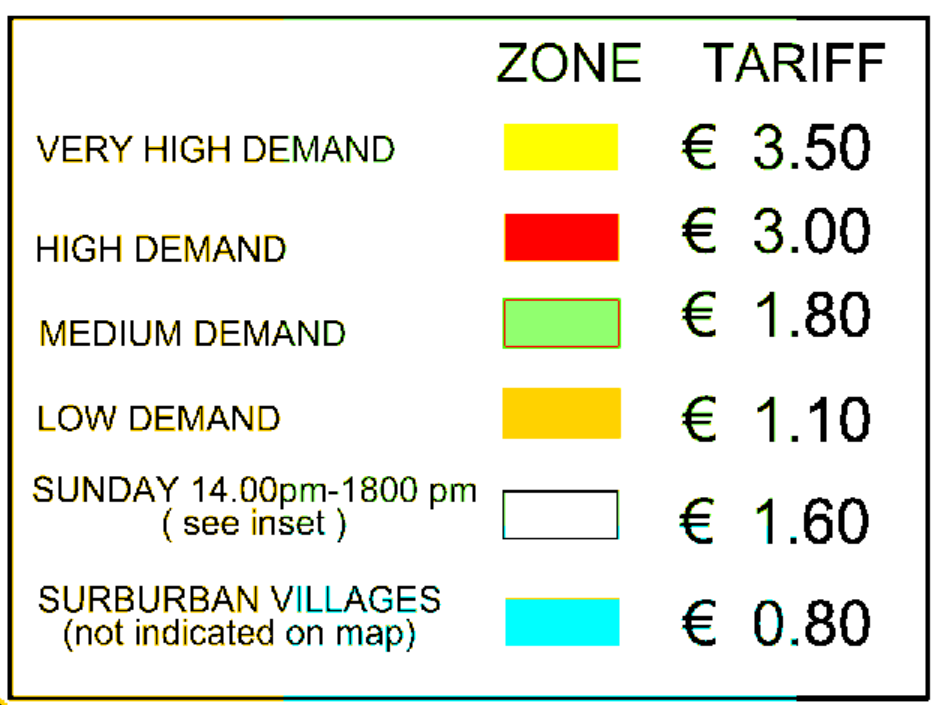
\includegraphics[width=\textwidth]{images/Parking_zones_cost.png}
  \end{minipage}
  \caption{Parking zones and cost defined by Dublin City Council}
  \label{fig:Parking_zones}
\end{figure}

Lastly, the csv file containing the longitude, latitude, classification label, parking
zone and parking cost is then uploaded to the PostgreSQL database, in the
backend server using the \texttt{send\_points.py} script.

\newpage{}

\subsubsection{Summary of main challenges}
Throughout the implementation of our technical solution, there have been many
major challenges and changes throughout the project timeline.

\textbf{Week 1-4}
This iteration focused on the startup of the project, exploratory work, machine
learning model tryouts and setting up Magpie's environment.

The biggest initial
hurdle was finding a labelling software to annotate our satellite images.
Initially, we had settled on LabelImg, however it was no longer being supported
on most of our operating systems and was crashing on launch. Instead, we turned
towards Label Studio and the ML Backend extension, which we intended on using
for its active learning functionality that would have enabled using YOLO v5 to
automatically label our training images, after only annotating a few images.
After much unsuccessful troubleshooting, we decided to switch approaches to
manually label the images and subsequently train the YOLO model on those images.

The next challenge related to training the YOLO model to identify cars on the
satellite images. An object detection model remains a deep neural network model,
which is computationally intensive the more complex it becomes.

We were limited in our training of the model due to limitations in available
computational resources. Tuning for 35 iterations would last several hours, and
training above a certain number of epochs would not yield better results.
Training the model was both computationally expensive and very time consuming.

Another challenge referred to the low resolution of the satellite images,
heavily contributing to the high misclassification rate in the early beginnings of
model training. We managed to stabilised that through proper model choosing and
tuning however, the biggest factor contributing to the remaining false positive
rate is the low number of training data.

Ideally we would've preferred to have at least 500 training images, however due
to time constraints we settled on half of that, and compensated by putting a
higher confidence threshold than the one dictated by the F1-curve.

\textbf{Week 5-8}

Another major challenge, was the unoccupied parking detection section. The key
decisions and changes are recounted below, following the timeline of our
project:

In Week 8, the \texttt{parking\_detection.py} script was updated to use the most
up to date trained YOLO model, YOLO v8 obb, that returned oriented bounding
boxes, causing many issues in the version of our script at the time,
specifically the way of accessing the bounding boxes predicted by the model had
changed. Furthermore, given the change to oriented bounding boxes, the size of
the bounding boxes became more variable, which allowed the script to be adapted
to use average parking spot dimensions.

\textbf{Week 9-12}

Week 9 was decisive in implementing a double pass-through to sort the cars by
longitude and the latitude to identify both the horizontal and vertical spots.
Moreover, the \texttt{parking\_detection.py} script was updated to use the
xywhr(centre coordinates, width, height and rotation) bounding boxes instead of
the xyxy (top left, bottom right)  bounding boxes we were using initially. This
major change was crucial, adding more modularity and allowing the
separation into horizontal and vertical cases in a more consistent manner.
Many additional improvement were made that week, such as the removal of
overlapping spots and filtering out the empty spots detected on the road.

In week 12, the unoccupied parking detection was completely finalized, resolving the
majority of the outstanding issues.\\
Originally 4 cases were considered, cars parked horizontally in a row or in a
column, cars parked vertically in a column and cars parked vertically side by
side. However, horizontally parked in a column and vertically parked side by side
were removed as they led to too many misclassifications, namely the vertically
parked side by side lead to adding many additional cars in driveways in
residential areas.
Additionally the condition on the angle alignment was refined and added to ensure
the detection of spots only between cars properly aligned.

Another major issue was the selection and accurate labelling of the test sets to
evaluate each subpart of our model.\\
Week 11 marked the beginning of the unoccupied parking detection evaluation. 
Labelling the test set accurately was a significant challenge, multiple different 
phases of relabelling and improvements occurred, to ensure the maximum overlap 
between the true labels and the model's predictions, achieving a high enough IoU.
The images were originally annotated using rotated bounding boxes, however due to the fact that
the rotation cannot be exported in Label Studio, they were subsequently relabelled without rotation.\\ 
During Week 12, the two other evaluation scripts were finalized. 
Similarly, multiple phases of labelling and relabelling occurred. For
the classification of spots evaluation, additional images containing private class instances
were added to the test set, as the initial lack of enough instances was making
that class perform poorly in comparison to the other classes.

\newpage{}